\section{Background}
\label{sec:background}

\subsection{LLM Inference Serving and Continuous Batching}
\label{subsec:serving}

Modern LLM serving engines process requests in \emph{iterations}: at each
decoding step, the engine advances every active sequence in the current batch
by one token, rather than running each request to completion before starting
the next. This scheme, continuous batching, lets new requests join a batch
and finished requests leave it between individual decoding steps, so GPU
compute is not left idle waiting for the longest sequence in a static batch
to finish. vLLM~\cite{kwon2023vllm}, the serving engine used in this work,
combines continuous batching with PagedAttention, a memory management scheme
that allocates the key-value cache in fixed-size, non-contiguous blocks,
avoiding the fragmentation of a pre-allocated maximum-length cache per
request and letting more concurrent sequences fit in a fixed amount of GPU
memory. Figure~\ref{fig:architecture_pipeline} illustrates where a
scheduling policy sits in this pipeline: it orders requests admitted into
the continuous-batching engine but does not alter the engine itself.

\begin{figure}[t]
    \centering
    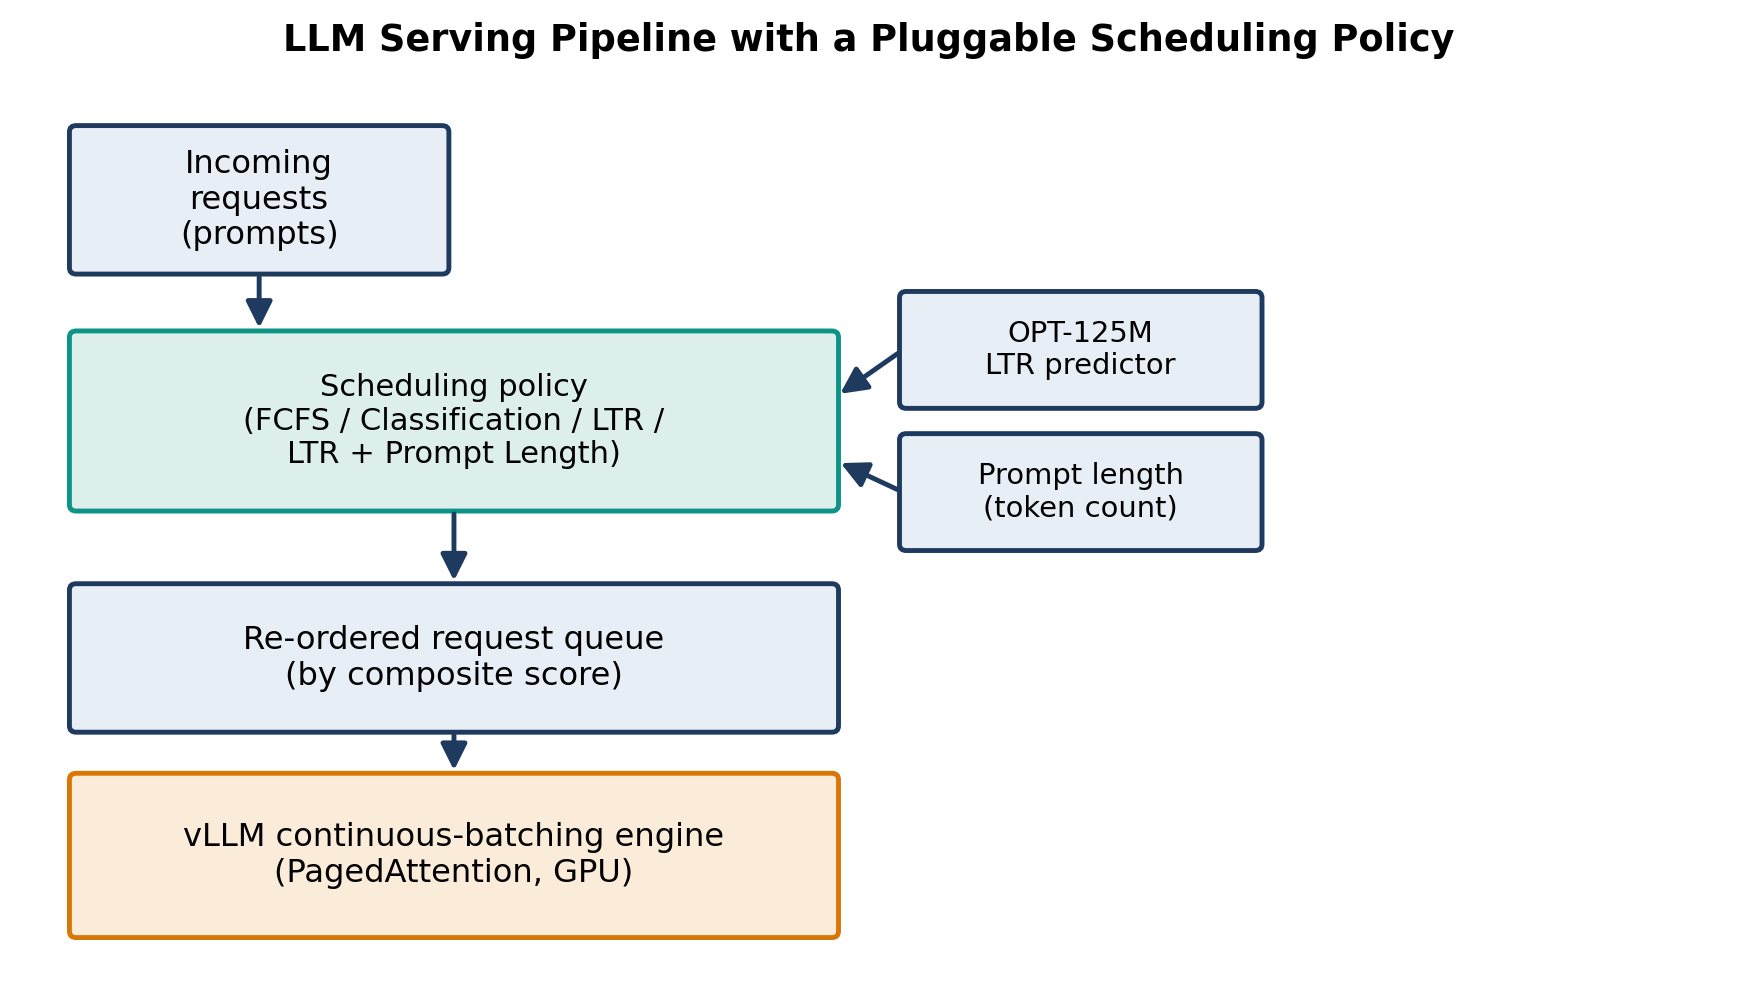
\includegraphics[width=0.95\linewidth]{figures/architecture_pipeline.png}
    \caption{LLM serving pipeline with a pluggable scheduling policy. The
    policy re-orders incoming requests before they are admitted to vLLM's
    continuous-batching engine; the engine itself is unmodified.}
    \label{fig:architecture_pipeline}
\end{figure}

\subsection{Head-of-Line Blocking Under Unknown Output Length}
\label{subsec:hol}

Continuous batching removes idle GPU time between requests, but it does not
by itself protect short requests from being scheduled behind long ones. If
the admission order is FCFS, a request that arrives early but will generate
hundreds of tokens occupies a batch slot for its full decoding duration, and
a request that arrives shortly after but would have finished in a few tokens
must still wait its turn. This is the LLM-serving analogue of HOL blocking:
the request at the head of the queue determines how long everything behind
it waits, regardless of how short that work actually is. Because output
length is not observable before decoding completes, mitigating HOL blocking
requires either estimating it in advance or using a proxy signal that
correlates with it.

\subsection{Learning-to-Rank Scheduling}
\label{subsec:ltr-background}

One way to estimate output length in advance is to train a small model to
predict it, or a value that ranks requests similarly to it, directly from the
prompt text. The LTR approach this work builds on fine-tunes a compact
OPT-125M model~\cite{zhang2022opt} with a ranking loss (ListMLE) so that its
output score orders requests consistently with their true relative output
lengths, rather than predicting the exact token count. Requests are then
admitted in order of this learned score, giving requests expected to be short
priority over requests expected to be long. This is effective to the extent
that the predictor's training distribution matches production traffic, but
the score is the predictor's only signal: if the prompt distribution shifts
or the predictor is uncertain, there is no independent signal to fall back
on. Prompt length is a natural candidate for such a fallback signal, since it
is known instantly and without any additional inference cost;
Figure~\ref{fig:composite_scoring} shows how it is combined with the learned
predictor score to form the composite ranking used in this work, whose
precise formulation is given in Section~\ref{sec:methodology}.

\begin{figure}[t]
    \centering
    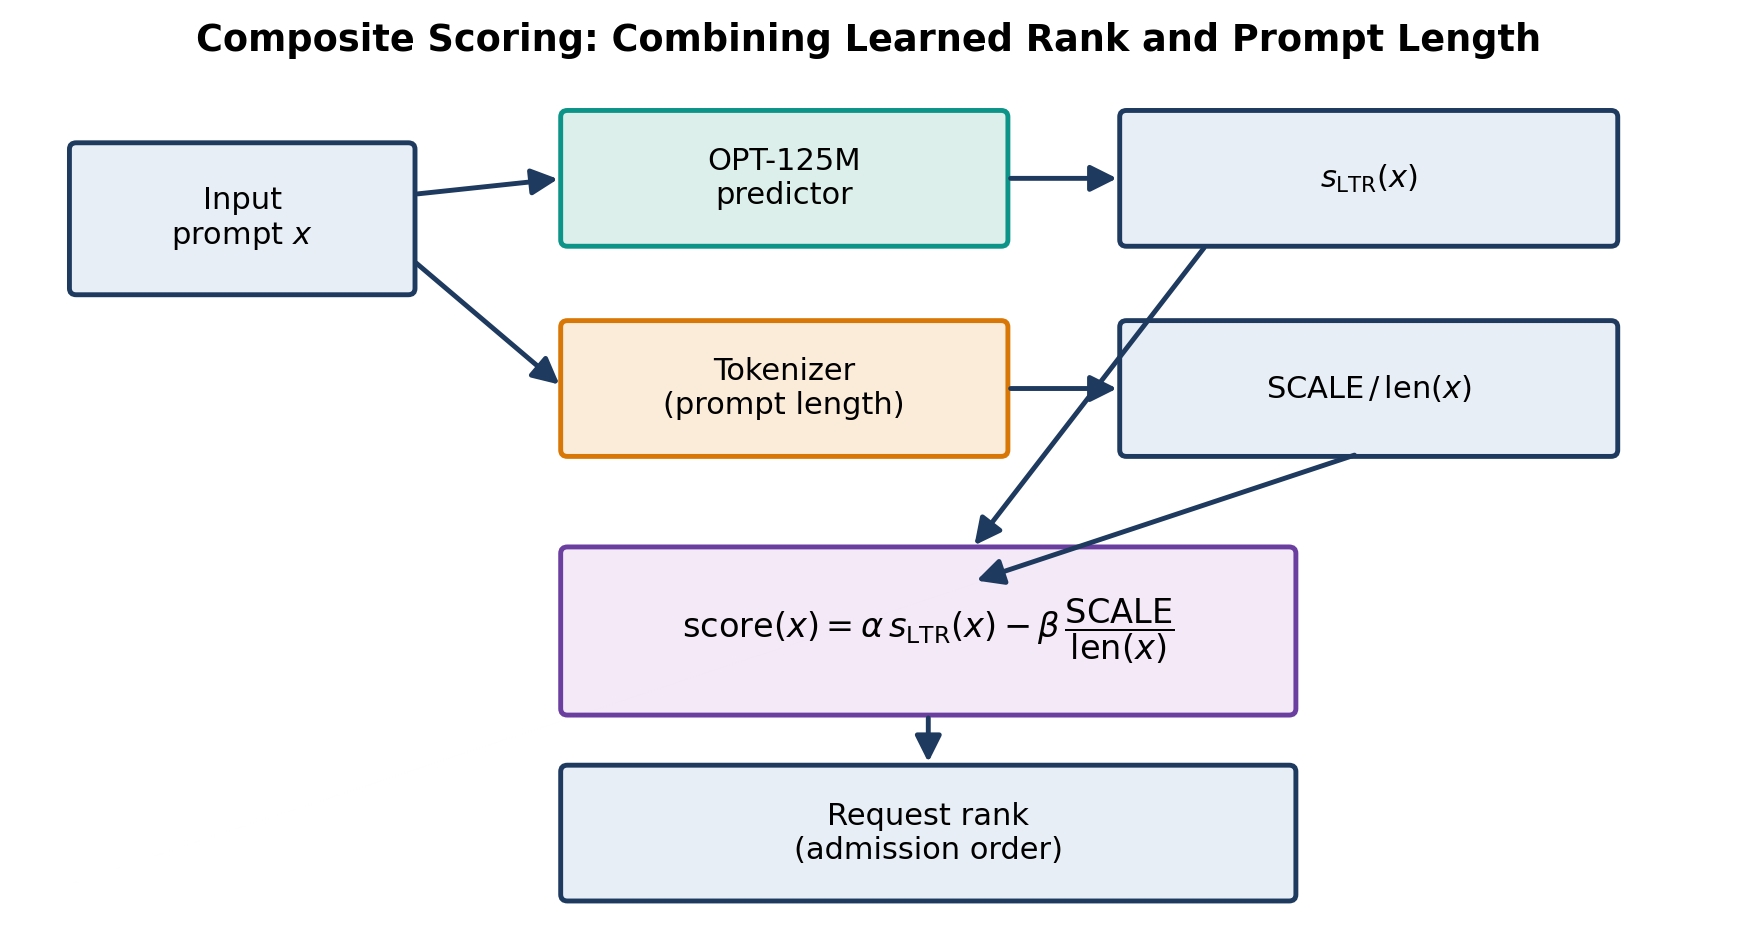
\includegraphics[width=0.95\linewidth]{figures/composite_scoring_architecture.png}
    \caption{Composite scoring architecture. The learned LTR predictor score
    and a normalized prompt-length term are combined into a single ranking
    score used to order the admission queue.}
    \label{fig:composite_scoring}
\end{figure}
